\section*{Abstract}


%Zielsetzung, Problemstellung
Die vorliegende Dokumentation beschreibt die Umsetzung des in Produktentwicklung 1 (PREN 1) entwickelten Konzepts. Der autonome Wegfindungsroboter wird im Rahmen des Moduls Produktentwicklung 2 (PREN 2) an der Hochschule Luzern gebaut und getestet. Der Roboter muss in der Lage sein autonom ein linienbasiertes Wegenetz zu durchqueren, Hindernisse zu erkennen und zu versetzen sowie einen zuvor definierten Zielknoten anhand von Bildverarbeitung zuverlässig zu finden. Die Risikobewertung und die Sprintplanung dienen als zentrale Projektmanagement Tools.  

% Methoden
Ausgehend von der Produktbeschreibung werden die einzelnen Systemkomponenten am fertigen System implementiert. Erkenntnisse aus Testaufbauten aus PREN 1 wurden berücksichtigt. Wurde vom ursprünglichen Konzept abgewichen wird darauf konkret eingegangen und begründet. 

Eine Herausforderung war das korrekte Auslesen der Encoder-Motoren die für die Drehung des Roboters verantwortlich sind. Für die exakte Drehung zu bestimmen wurde schliesslich ein Gyroskop verwendet. Die Steuerung des Roboters erfolgt durch eine Kombination aus dem Mikrocontroller Tiny K22 für zeitkritische Steueraufgaben und einem Raspberry Pi für die Bildverarbeitung und Navigation. Während der Implementierung und dem Testen wurden erkannte Probleme durch iterative Anpassungen minimiert.

% Ergebnissse

Die Implementierung des Gyroskop für die Regelung des Drehwinkels konnte abgeschlossen werden. Trotz aller funktionierender Einzelkomponenten konnte das Gesamtsystem zum Zeitpunkt der Abgabe die komplette Aufgabe nicht erfolgreich abschliessen, da noch an der Systemintegration gearbeitet wird. Es wurden im Vorfeld viele Tests für die Navigation durchgeführt was das die Systemintegration erleichtert.

% Ausblick
Obwohl das Gesamtsystem zum Zeitpunkt der Abgabe nicht funktionierte, kann davon ausgegagen werden das der Roboter die Aufgabenstellung selsbständig bewältigen kann. Die Arbeit eine solide Grundlage für das Entwickeln von Prototypen in interdisziplinärer Arbeit. Die gesammelten Erfahrungen sind Wertvoll für zukünftige Projekte im akademischen Umfeld sowie in der Arbeitswelt.


\begin{figure}[h]
    \centering
    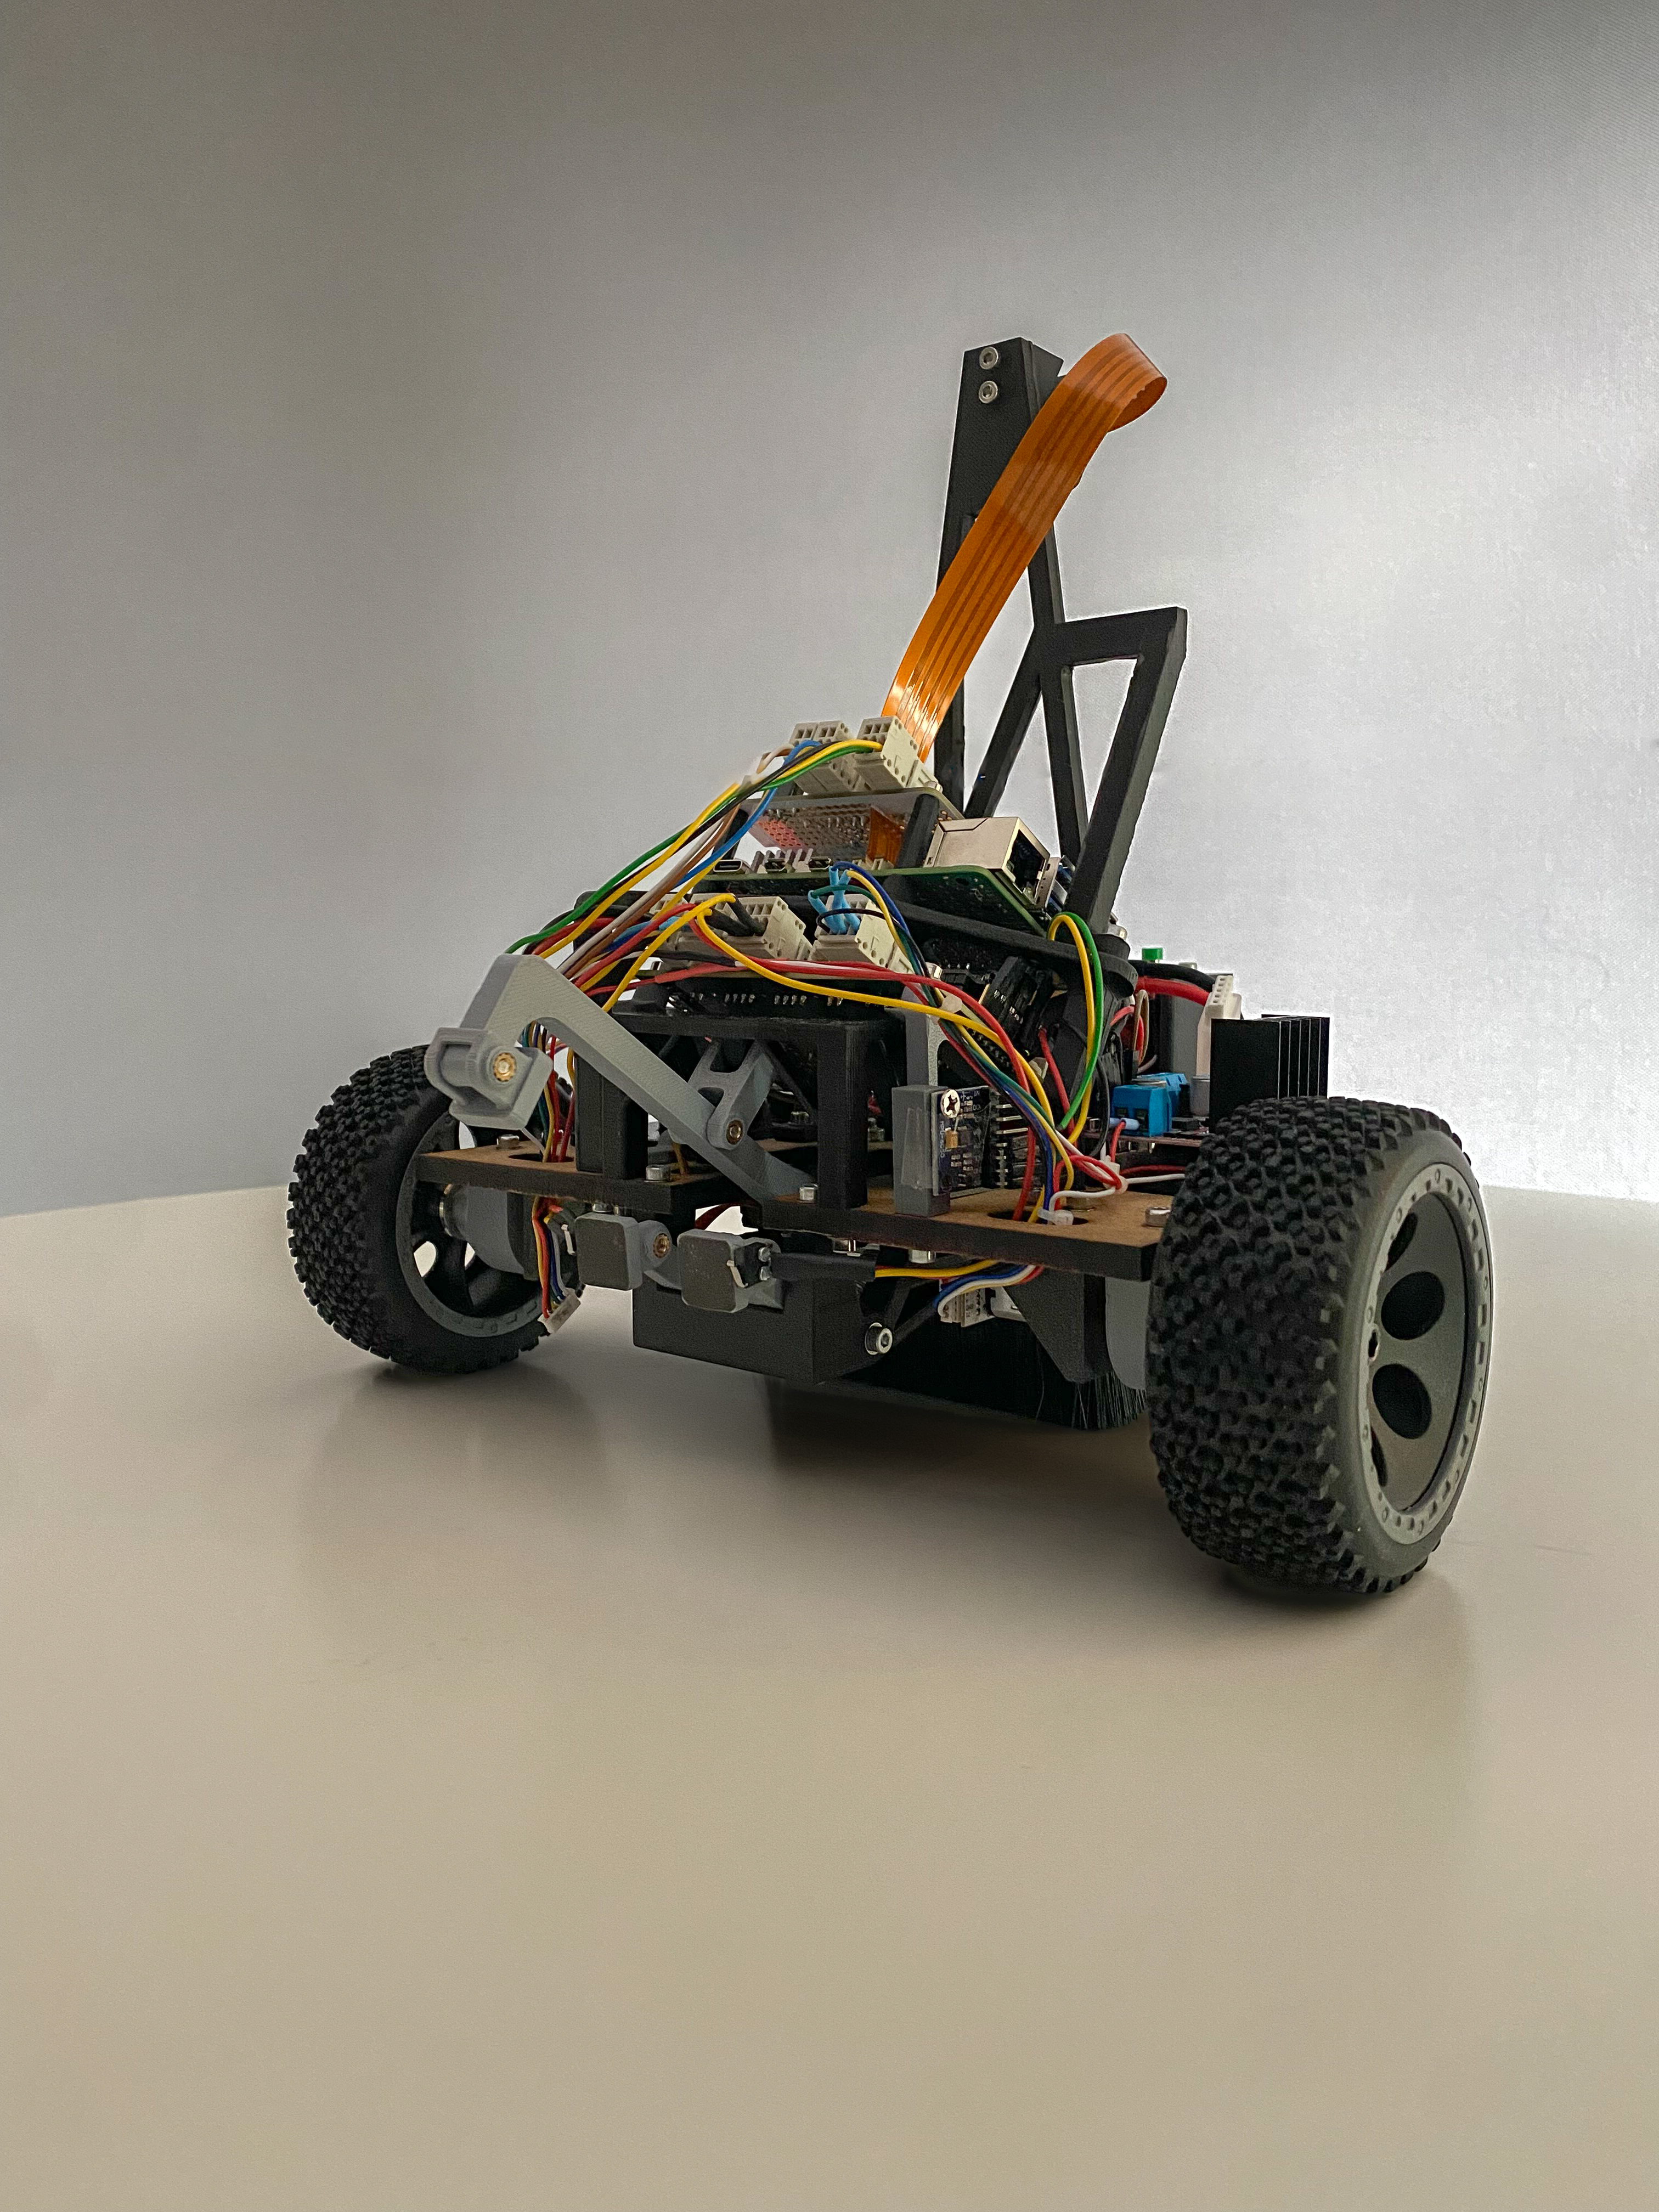
\includegraphics[width=0.4\textwidth, trim={0cm 7cm 0cm 2cm}, clip]{assets/PREN2_Roboter_back.jpg}
    \caption{Rückansicht des Roboters}
    \label{fig:roboter_back}
\end{figure}


